\subsection{Structures in (re-)entry vehicles}\label{sec:struc}
Applications and technologies, within the field of structures and materials, as applied in (re-)entry vehicles are investigated, with an emphasis on inflatable aeroshells. These are investigated firstly for non-inflatable structures and secondly for inflatable structures.

\subsubsection{Non-inflatable structures}
Non-inflatable structures can be either deployable or non-deployable. Conventional solutions, such as the Apollo or Soyuz capsule, employ a non-deployable heat shield. An advantage of a deployable heat shield is effecting a larger surface area for aerodynamic deceleration. In most cases, this is supplemented by retropropulsive means.



\subsubsection{Inflatable structures}
The inflatable aeroshell system implemented in the \gls{irve} satellites mainly consists of four sub-elements: an inflatable bladder, containing a pressurised medium, a structural restraint, gas barrier and a thermal protection layer \cite{Hughes2005}. In addition, this bladder may be further subdivided into isolated volumes to provide avoid \gls{spfs}. After flow initiation with pyrotechnic valves the gas flows from the storage tank to the inflatable bladder. This flow is protected by gas valves to prevent backflow from the bladders. \cite{Hughes2005} 

In terms of the inflation process, the pressure and gas used for inflation are variable. The IRVE satellites featured nitrogen gas (and subliming powders), with an operating pressure of 3000 psi for IRVE-4 \cite{Litton2011}. An alternative to the use of nitrogen gas is hydrazine, typically capable of delivering lower weight and volume, at the expense of handling, safety and cost \cite{Freeland1998}. Estimating the required minimum pressure can be done using references \cite{Samareh2011, Brown2009}.

An alternative to using a pressurised gas is the use of the local atmosphere, so-called ram-air inflation. This can be achieved by outfitting the aeroshell with inlets that allows high dynamic pressure freestream air to inflate it. This does, however, limit deployment to within the atmosphere, where the dynamic pressure is adequately high. Extending inflation possibilities can be done by using a hybrid, therefore using both an internal gas source and ram-air inflation. \cite{Smith2010}

In addition to pure inflation, rigidization may be applied. Rigidization stiffens the structure after inflation, a process that may be performed by multiple techniques. These techniques are described in references \cite{Freeland1998,Jenkins2001}, for example using fibres impregnated with a resin that cures at a certain temperature. 

The structural load is carried by the bladder walls and may in addition be partly carried by support straps (radial direction) and gores (circumferential direction). Calculating the loads for inflatable structures can be done using membrane theory, as per Ref. \cite{Young2002}. Structural analysis and testing as applied to an inflatable aeroshell is described in Ref. \cite{Lindell2006}.

Materials used for \gls{hiad} are typically textile materials, such as Kevlar, Vectran and Zylon. For example, IRVE-II and IRVE-III used Kevlar fibres, with a silicone coating \cite{Dillman2012a}. \gls{thor} replaced the Kevlar by Zylon \footnote{Pro Fiber Zylon Technical Information. \\ URL: \url{http://www.toyobo-global.com/seihin/kc/pbo/Technical\_Information\_2005.pdf}. Accessed 24 April 2015} fibres for their retainment of (usable) strength at high temperature (400 degrees Celsius versus 250 degrees Celsius) \cite{Dillman2014}. An overview of materials used in membrane structures in space is given by Ref. \cite{Jenkins2001}. Figure \ref{fig:matlayup} presents an overview of the material lay-up used for the bladder walls of IRVE-II.

\begin{figure}[H]
\centering
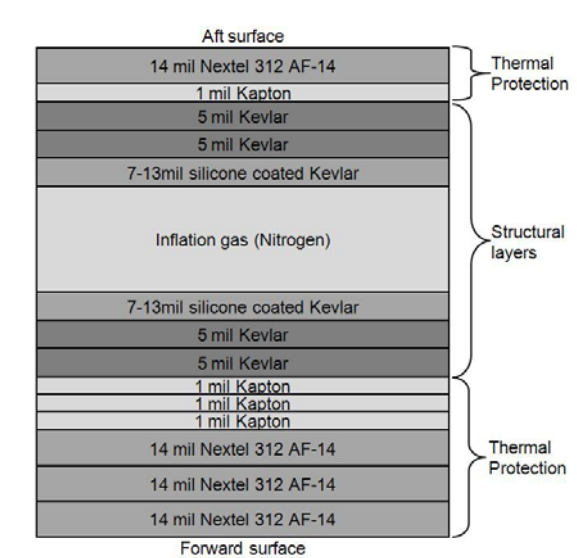
\includegraphics[width = 0.4\textwidth]{Figure/IRVE2_bladder_mat.PNG}
\caption{Bladder wall material lay-up of inflatable volume walls. From \cite[p.2]{Dillman2010}}
\label{fig:matlayup}
\end{figure}

A number of configurations exists for an aerodynamic decelerator \cite{Smith2010}. While the discussion on aeroshell shape is limited to Chapter \ref{cha:design}, only references for specific (structural) analysis are hereafter given. For a tension cone Ref. \cite{Yamada2009} provides an entry for structural analysis and design; for an isotensoid Ref. \cite{Smith2011}; for a stacked toroid configuration the IRVE satellites provide good reference material. It should be noted that there is a trend towards the use of \gls{fem} in structural analysis and design, but that in view of current team member knowledge and experience this is not a feasible alternative.













